\documentclass[letterpaper]{article}
\usepackage{amsmath,amssymb}
\usepackage{lmodern}
\usepackage{iftex}

\usepackage[T1]{fontenc}
\usepackage[utf8]{vietnam}
\usepackage{textcomp} % provide euro and other symbols
\usepackage{lipsum}
\usepackage{setspace}
\usepackage{hyperref}
\usepackage{xcolor}
\usepackage[table]{xcolor}
\usepackage{longtable,booktabs,array}
\usepackage{multirow}
\usepackage{calc} % for calculating minipage widths
% Correct order of tables after \paragraph or \subparagraph
\usepackage{etoolbox}

\usepackage{adjustbox}
\usepackage{graphicx}
\makeatletter
\def\maxwidth{\ifdim\Gin@nat@width>\linewidth\linewidth\else\Gin@nat@width\fi}
\def\maxheight{\ifdim\Gin@nat@height>\textheight\textheight\else\Gin@nat@height\fi}
\makeatother
% Scale images if necessary, so that they will not overflow the page
% margins by default, and it is still possible to overwrite the defaults
% using explicit options in \includegraphics[width, height, ...]{}
\setkeys{Gin}{width=\maxwidth,height=\maxheight,keepaspectratio}

\usepackage{tabularx}
% \setlength{\parskip}{1cm plus 4mm minus 3mm}
% \setlength{\parindent}{1cm}
\usepackage[top=15mm, bottom=15mm, left=30mm, right=30mm]{geometry} % page layout

% add biblatex
\usepackage[backend=bibtex,style=numeric ,natbib=true, sorting=nty, maxbibnames=99]{biblatex} 
\addbibresource{ref}

% re-define section/ subsection
\usepackage{titlesec}
\providecommand{\tightlist}{%
  \setlength{\itemsep}{0pt}\setlength{\parskip}{0pt}}
\setcounter{secnumdepth}{-\maxdimen} % remove section numbering
\DeclareUnicodeCharacter{0301}{*************************************}

\titleformat{\section}
  {\large\bfseries\color{blue}}
  {\thesection}{1em}{}
\titleformat{\subsection}
  {\large\bfseries\color{blue}}
  {\thesection}{1em}{}
\titleformat{\subsubsection}
  {\normalsize\color{blue}}
  {\thesection}{1em}{}
\author{Khoa Nguyen}
\date{Oct 2023}

\begin{document}

\begin{table*}[!ht]
    \centering
    \begin{tabular}{m{6em} c  m{7em} m{5em} }
   

         \multirow{3}{3em}{
         \begin{minipage}{0.15\textwidth}
      \includegraphics{asset/Figure/image1.png}
    \end{minipage}} & 
     & & \\  \cline{3-4}
     & \small ĐẠI HỌC QUỐC GIA TP.HCM &  \multicolumn{1}{|c|}{\multirow{2}{8em}{\small Ngày nhận hồ sơ}} &  \multicolumn{1}{|c|}{}\\
    & \small \textbf{TRƯỜNG ĐẠI HỌC CÔNG NGHỆ THÔNG TIN} & \multicolumn{1}{|c|}{} &  \multicolumn{1}{|c|}{}\\\cline{3-4}

        & & \multicolumn{2}{|c|}{\textit{\small (Do CQ quản lý ghi)}}\\ \cline{3-4}
    
    \end{tabular}
    % \caption{Caption}
    % 
\end{table*}

\begin{quote}
\centering
\textbf{\Large THUYẾT MINH}

\Large ĐỀ TÀI NGHIÊN CỨU KHOA HỌC SINH VIÊN 2025
\end{quote}


\section{A. THÔNG TIN CHUNG}

\subsection{A1. Tên đề tài}


\begin{itemize}
\item[-]  Tên tiếng Việt (IN HOA): HỆ THỐNG MẠNG LƯỚI ĐIỀU KHIỂN ĐÈN GIAO THÔNG THÔNG
MINH SỬ DỤNG DEEP REINFORCEMENT LEARNING VÀ IOT
\item[-]  Tên tiếng Anh (IN HOA): INTELLIGENT TRAFFIC LIGHT CONTROL NETWORK SYSTEM
USING DEEP REINFORCEMENT LEARNING AND IOT 
\end{itemize}


\subsection{A2. Thời gian thực hiện}

6 tháng (kể từ khi được duyệt).

\subsection{A3. Tổng kinh phí}

\noindent Tổng kinh phí: 6 triệu đồng.

% \begin{itemize}
% \item
%   Kinh phí từ Trường Đại học Công nghệ Thông tin: 6 triệu
%   đồng
% \end{itemize}


\subsection{A4. Chủ nhiệm}
\begin{spacing}{1.5}

\indent \indent Họ và tên: Đặng Nguyễn Hoàng Phúc\par

Ngày, tháng, năm sinh: 18/07/2003 \hspace{2cm} Giới tính (Nam/Nữ): Nam\par

Số CCCD: 095203008556\hspace{3.5cm} Ngày cấp: 31/05/2021\par Nơi cấp: Cục cảnh sát QLHC về TTXH\par

Mã số sinh viên: 21522470

Số điện thoại liên lạc: 0378205920

Khoa: Mạng máy tính và Truyền thông\par

Số tài khoản: 9378205920\hspace{2cm} Ngân hàng: Vietcombank chi nhánh Hùng Vương
\end{spacing}

\subsection{A5. Thành viên đề tài (kể cả CNĐT)}

\textbf{\color{red}Chỉnh lại độ rộng các cột cho vừa với text}

\begin{longtable}[c]{@{}
  >{\raggedright\arraybackslash}p{(\columnwidth - 6\tabcolsep) * \real{0.0553}}
  >{\raggedright\arraybackslash}p{(\columnwidth - 6\tabcolsep) * \real{0.3235}}
  >{\raggedright\arraybackslash}p{(\columnwidth - 6\tabcolsep) * \real{0.3637}}
  >{\raggedright\arraybackslash}p{(\columnwidth - 6\tabcolsep) * \real{0.2575}}@{}}
\toprule()
\begin{minipage}[b]{\linewidth}\raggedright
\textbf{TT}
\end{minipage} & \begin{minipage}[b]{\linewidth}\raggedright
\textbf{Họ tên}
\end{minipage} & \begin{minipage}[b]{\linewidth}\raggedright
\textbf{MSSV}
\end{minipage} & \begin{minipage}[b]{\linewidth}\raggedright
\textbf{Khoa}
\end{minipage} \\
\midrule()
\endhead
1 & Đặng Nguyễn Hoàng Phúc & 21522470 & Mạng máy tính và Truyền thông\\
2 & Nguyễn Thanh Duy & 21520780 & Mạng máy tính và Truyền thông\\
\bottomrule()
\end{longtable}



\section{B. MÔ TẢ NGHIÊN CỨU}

\textbf{\color{red}Phần này mô tả bài toán và related works, sau đó đưa ra hướng giải quyết của mình. Sau đó Phần Giới thiệu về đề tài mô tả tóm gọn mục tiêu/cách thức mình giải quyết bài toán}

\indent \indent Nghiên cứu này đề xuất một hệ thống mạng lưới điều khiển đèn giao thông thông minh sử dụng Deep Reinforcement Learning (DRL) và Internet of Things (IoT). Hệ thống tận dụng dữ liệu thời gian thực từ camera giám sát, kết hợp với các thuật toán học tăng cường sâu để tối ưu hóa việc điều khiển đèn giao thông, nhằm giảm thiểu thời gian chờ đợi và tăng hiệu quả lưu thông trên toàn mạng lưới giao thông.

\subsection{B1. Giới thiệu về đề tài}

Sự phát triển nhanh chóng của các đô thị thông minh đã đặt ra nhiều thách thức trong quản lý và điều khiển giao thông đô thị. Các phương pháp điều khiển đèn giao thông truyền thống dựa trên thời gian cố định không còn đáp ứng được nhu cầu ngày càng phức tạp của giao thông đô thị hiện đại. Theo nghiên cứu của Cesme và Urbanik \cite{cesme2021signal}, việc thiếu sự phối hợp giữa các nút giao thông là nguyên nhân chính dẫn đến tình trạng tắc nghẽn cục bộ và làm giảm hiệu quả chung của toàn hệ thống.

Xu hướng mới trong quản lý giao thông là sử dụng các hệ thống thông minh có khả năng tự học và thích nghi. Gao và cộng sự \cite{gao2017adaptive} đã chứng minh rằng việc áp dụng học tăng cường vào điều khiển đèn giao thông có thể giảm thời gian chờ đợi trung bình xuống khoảng 40\% so với các phương pháp truyền thống. Tuy nhiên, các nghiên cứu hiện tại vẫn tồn tại những hạn chế đáng kể:

\begin{itemize}
    \item Phần lớn các nghiên cứu chỉ tập trung vào điều khiển các nút giao thông riêng lẻ mà không xem xét tương tác giữa các nút \cite{yasa2024reducing}.
    \item Các thách thức về xử lý dữ liệu thời gian thực và đồng bộ hóa giữa các nút vẫn chưa được giải quyết triệt để \cite{el2014design}.
    \item Có rất ít hệ thống tích hợp cả công nghệ IoT và Deep Reinforcement Learning trong một giải pháp toàn diện \cite{aradi2020survey}.
\end{itemize}

\begin{figure}[!hbt]
    \centering
    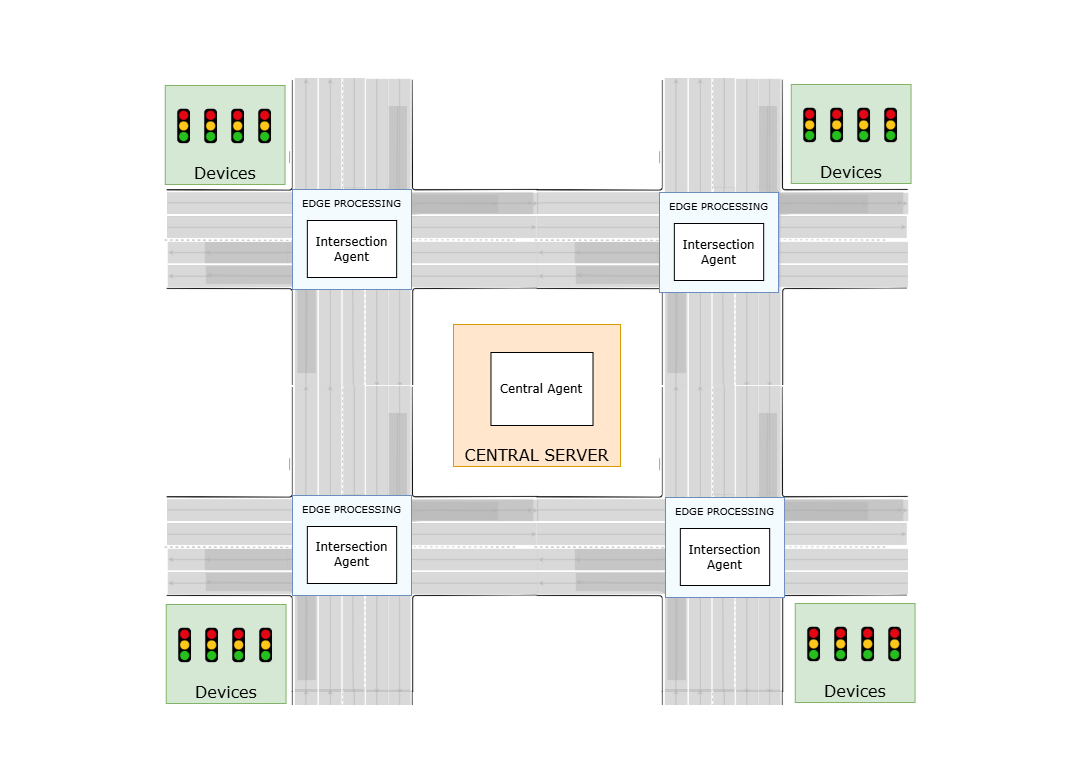
\includegraphics[width=0.8\textwidth]{Figures/overview_architecture.png}
    \caption{Kiến trúc tổng thể của hệ thống điều khiển đèn giao thông thông minh}
    \label{fig:sys-arch}
\end{figure}

Nghiên cứu này đề xuất một hệ thống mới (Hình \ref{fig:sys-arch}) nhằm khắc phục những hạn chế trên bằng cách kết hợp dữ liệu thu thập từ hệ thống camera với các thuật toán học tăng cường sâu, tạo ra một hệ thống điều khiển đèn giao thông thông minh, tự động và có khả năng điều phối nhiều nút giao thông cùng lúc.

\subsection{B2. Mục tiêu, nội dung, kế hoạch nghiên cứu}

\subsection{B2.1 Mục tiêu}

Mục tiêu tổng thể của đề tài là phát triển hệ thống mạng lưới điều khiển đèn giao thông thông minh có khả năng tối ưu hóa luồng giao thông và giảm thiểu tắc nghẽn trên nhiều giao lộ. Cụ thể:

\begin{itemize}
    \item Xây dựng và huấn luyện mô hình Deep Reinforcement Learning để điều khiển đèn giao thông thời gian thực, với khả năng tự học và thích nghi với các điều kiện giao thông khác nhau.
    \item Phát triển hệ thống trích xuất thông tin thời gian thực từ camera giám sát, cung cấp dữ liệu đầu vào chính xác cho mô hình.
    \item Thiết kế và triển khai cơ chế phối hợp giữa các nút giao thông, tạo thành mạng lưới điều khiển đồng bộ.
    \item Xây dựng giao diện người dùng trực quan, cung cấp thông tin giao thông và trạng thái hệ thống, hỗ trợ cho việc điều khiển và giám sát.
    \item Đánh giá hiệu quả của hệ thống thông qua các chỉ số về thời gian di chuyển, độ trễ và lưu lượng giao thông.
\end{itemize}

\subsection{B2.2 Nội dung và phương pháp nghiên cứu}

\subsubsection{Nội dung 1: Nghiên cứu tổng quan về điều khiển đèn giao thông và học tăng cường sâu}

\paragraph{Phương pháp thực hiện:}
\begin{itemize}
    \item Tiến hành tổng hợp và phân tích các nghiên cứu liên quan đến điều khiển đèn giao thông thông minh và ứng dụng của học tăng cường.
    \item Khảo sát các giải pháp hiện có, đánh giá ưu nhược điểm của từng phương pháp.
    \item Xác định các khoảng trống nghiên cứu và đề xuất hướng tiếp cận mới.
    \item Xây dựng kiến trúc hệ thống chi tiết bao gồm các thành phần chính như mô hình DRL, hệ thống IoT và giao diện người dùng.
\end{itemize}

\paragraph{Kết quả dự kiến:}
\begin{itemize}
    \item Báo cáo tổng quan về tình hình nghiên cứu hiện tại trong lĩnh vực điều khiển đèn giao thông thông minh.
    \item Khung lý thuyết cho việc áp dụng Deep Reinforcement Learning vào hệ thống điều khiển đèn giao thông.
    \item Kiến trúc tổng thể của hệ thống kết hợp IoT và Deep Reinforcement Learning.
\end{itemize}

\subsubsection{Nội dung 2: Phát triển mô hình Deep Reinforcement Learning}

\paragraph{Phương pháp thực hiện:}
\begin{itemize}
    \item Xây dựng mô hình toán học cho bài toán điều khiển đèn giao thông, bao gồm định nghĩa về trạng thái, hành động và phần thưởng.
    \item Thiết kế mạng nơ-ron sâu cho thuật toán Deep Q-Learning dựa trên kiến trúc CNN như Hình \ref{fig:drl-model}.
    \item Phát triển môi trường mô phỏng giao thông để huấn luyện và đánh giá mô hình.
    \item Huấn luyện mô hình DRL trên môi trường mô phỏng với các kịch bản giao thông khác nhau.
    \item Tối ưu hóa tham số mô hình để đảm bảo hiệu quả điều khiển cao.
\end{itemize}

\begin{figure}[!hbt]
    \centering
    \includegraphics[width=0.7\textwidth]{Figures/drl_model.png}
    \caption{Mô hình học tăng cường sâu cho hệ thống điều khiển đèn giao thông \cite{kovari2022deep}}
    \label{fig:drl-model}
\end{figure}

\paragraph{Kết quả dự kiến:}
\begin{itemize}
    \item Mô hình Deep Q-Learning được tối ưu hóa cho điều khiển đèn giao thông.
    \item Môi trường mô phỏng giao thông đô thị với nhiều giao lộ.
    \item Đánh giá hiệu quả của mô hình trên các kịch bản khác nhau.
    \item So sánh hiệu suất với các phương pháp điều khiển truyền thống.
\end{itemize}

\subsubsection{Nội dung 3: Phát triển hệ thống xử lý hình ảnh và trích xuất thông tin từ camera}

\paragraph{Phương pháp nghiên cứu:}
\begin{itemize}
    \item Thiết lập hệ thống camera giám sát tại các vị trí chiến lược.
    \item Phát triển module xử lý hình ảnh dựa trên mô hình YOLO để nhận diện và phân loại phương tiện giao thông.
    \item Xây dựng thuật toán theo dõi đối tượng để đo lường các thông số giao thông như mật độ, tốc độ và luồng di chuyển.
    \item Tích hợp các công nghệ xử lý đám mây để đảm bảo khả năng xử lý real-time.
    \item Xây dựng pipeline dữ liệu từ camera đến hệ thống xử lý trung tâm.
\end{itemize}

\paragraph{Kết quả dự kiến:}
\begin{itemize}
    \item Hệ thống camera giám sát được tối ưu hóa cho việc thu thập dữ liệu giao thông.
    \item Module nhận diện phương tiện với độ chính xác cao (>90\%).
    \item Pipeline xử lý dữ liệu thời gian thực với độ trễ thấp (<100ms).
    \item Khả năng trích xuất các thông số giao thông quan trọng từ video.
\end{itemize}

\subsubsection{Nội dung 4: Tích hợp mô hình DRL với dữ liệu thời gian thực}

\paragraph{Phương pháp nghiên cứu:}
\begin{itemize}
    \item Thiết kế cơ chế kết nối để đưa dữ liệu thời gian thực từ camera vào hệ thống.
    \item Phát triển kiến trúc đa tác tử (multi-agent) cho điều khiển phối hợp giữa nhiều giao lộ \cite{foerster2018deep}.
    \item Xây dựng cơ chế đồng bộ hóa giữa các mô hình RL tại các nút giao thông khác nhau.
    \item Thiết kế thuật toán học online để mô hình có thể liên tục cải thiện dựa trên phản hồi từ môi trường thực.
    \item Tối ưu hóa hiệu suất tính toán để đảm bảo khả năng đáp ứng thời gian thực.
\end{itemize}

\paragraph{Kết quả dự kiến:}
\begin{itemize}
    \item Hệ thống tích hợp hoàn chỉnh giữa mô hình DRL và dữ liệu camera thời gian thực.
    \item Kiến trúc đa tác tử cho điều khiển phối hợp giữa các giao lộ.
    \item Cơ chế học online với khả năng thích nghi nhanh với thay đổi giao thông.
    \item Đánh giá hiệu quả của hệ thống trên dữ liệu thực.
\end{itemize}

\subsubsection{Nội dung 5: Phát triển giao diện điều khiển và hệ thống demo}

\paragraph{Phương pháp nghiên cứu:}
\begin{itemize}
    \item Thiết kế giao diện web trực quan hiển thị trạng thái giao thông theo thời gian thực.
    \item Xây dựng bản đồ trực quan hóa toàn bộ mạng lưới đèn giao thông.
    \item Phát triển các công cụ phân tích và báo cáo để đánh giá hiệu quả hệ thống.
    \item Thiết kế chức năng điều khiển thủ công để can thiệp khi cần thiết.
    \item Xây dựng hệ thống demo hoàn chỉnh để trình diễn khả năng của giải pháp.
\end{itemize}

\paragraph{Kết quả dự kiến:}
\begin{itemize}
    \item Giao diện web giám sát trạng thái giao thông theo thời gian thực.
    \item Bản đồ trực quan hóa mạng lưới đèn giao thông với các chỉ số hiệu suất.
    \item Các công cụ phân tích và báo cáo cho việc đánh giá hệ thống.
    \item Hệ thống demo hoàn chỉnh để trình diễn giải pháp.
\end{itemize}

\subsection{B2.3 Kế hoạch nghiên cứu}

\textbf{\color{red}Phần này cần vẽ biểu đồ gantt thể hiện khoảng thời gian thực hiện các Nội dung bên trên, tham khảo bảng bên dưới}

\begin{table}[htbp]
\centering
\begin{tabular}{|c|c|c|c|c|c|c|}
\hline
Giai đoạn & Tháng 1 & Tháng 2 & Tháng 3 & Tháng 4 & Tháng 5 & Tháng 6 \\
\hline
Nội dung 1 & \cellcolor [rgb]{1,0,0}  &  &  & &  & \\
\hline
Nội dung 2 & & \cellcolor [rgb]{1,0.647,0} &  &  &  &  \\
\hline
Nội dung 3 & &  & \cellcolor[rgb]{1,1,0	} & \cellcolor[rgb]{1,1,0} &  &  \\
\hline
Nội dung 4 &  &  &  & \cellcolor[rgb]{0,1,1	} & \cellcolor[rgb]{0,1,1	} & \\
\hline
Nội dung 5 &  &  &  &\cellcolor[rgb]{0,1,0}  &\cellcolor[rgb]{0,1,0}  & \cellcolor[rgb]{0,1,0} \\
\hline
\end{tabular}
\caption{Bảng kế hoạch thực hiện đề tài}
\label{tab:plan}
\end{table}

Kế hoạch nghiên cứu được thực hiện trong khoảng thời gian từ 03/02/2025 đến 15/06/2025, với các giai đoạn chính như sau:

% \begin{table}[htbp]
%     \centering
%     \begin{tabular}{|p{3cm}|p{5cm}|p{5cm}|}
%         \hline
%         \textbf{Thời gian} & \textbf{Nội dung} & \textbf{Nhiệm vụ cụ thể} \\
%         \hline
%         03/02 - 13/02/2025 & Nghiên cứu và xây dựng kiến trúc hệ thống & - Xây dựng kiến trúc hệ thống\\
%         & & - Xây dựng môi trường mô phỏng cơ bản\\
%         \hline
%         13/02 - 02/03/2025 & Huấn luyện mô hình RL trên môi trường mô phỏng & - Phát triển mô hình RL cơ bản\\
%         & & - Huấn luyện mô hình với các kịch bản giao thông đơn giản\\
%         \hline
%         03/03 - 25/03/2025 & Tối ưu hóa mô hình RL, giao tiếp giữa các giao lộ & - Điều chỉnh tham số và cải thiện hiệu suất\\
%         & & - Thử nghiệm với các kịch bản phức tạp\\
%         & & - Huấn luyện giao tiếp giữa mô hình ở các giao lộ\\
%         \hline
%         26/03 - 05/04/2025 & Đồng bộ dữ liệu thực tế với mô phỏng & - Áp dụng cơ chế kết nối dữ liệu thực tế vào mô phỏng\\
%         & & - Đồng bộ hóa dữ liệu thời gian thực\\
%         \hline
%         05/04 - 03/05/2025 & Huấn luyện lại mô hình RL với dữ liệu thực tế & - Sử dụng dữ liệu thực tế để fine-tune mô hình\\
%         & & - Đánh giá hiệu suất mô hình trên dữ liệu thực\\
%         \hline
%         04/05 - 15/05/2025 & Xây dựng hệ thống điều khiển đèn theo thời gian thực & - Triển khai hệ thống đèn giao thông\\
%         & & - Đưa mô hình RL vào điều khiển đèn dựa trên dữ liệu thực\\
%         & & - Kiểm thử tính ổn định và độ trễ\\
%         \hline
%         15/05 - 01/06/2025 & Phát triển giao diện điều khiển và hiển thị & - Thiết kế giao diện người dùng (UI)\\
%         \hline
%         02/06 - 06/06/2025 & Kiểm thử toàn diện hệ thống & - Kiểm thử từng thành phần và toàn bộ hệ thống\\
%         & & - Đánh giá hiệu suất và độ ổn định\\
%         \hline
%         06/06 - 15/06/2025 & Triển khai thử nghiệm và báo cáo & - Triển khai thử nghiệm toàn hệ thống\\
%         & & - Tổng hợp kết quả và hoàn thiện báo cáo\\
%         \hline
%     \end{tabular}
%     \caption{Kế hoạch nghiên cứu chi tiết}
%     \label{tab:research-plan}
% \end{table}

\subsection{B3. Kết quả dự kiến}

Kết quả dự kiến của nghiên cứu bao gồm:

\begin{enumerate}
    \item \textbf{Hệ thống mô phỏng giao thông:} Môi trường mô phỏng đô thị với nhiều giao lộ, có khả năng mô phỏng các điều kiện giao thông khác nhau như giờ cao điểm, giờ thấp điểm và các tình huống khẩn cấp.
    
    \item \textbf{Mô hình Deep Reinforcement Learning:} Mô hình được huấn luyện để điều khiển đèn giao thông một cách tối ưu, có khả năng thích nghi với các điều kiện giao thông khác nhau và phối hợp giữa nhiều giao lộ.
    
    \item \textbf{Hệ thống trích xuất thông tin từ camera:} Module xử lý hình ảnh có khả năng nhận diện và phân loại phương tiện giao thông, trích xuất các thông số quan trọng như mật độ, tốc độ và luồng di chuyển.
    
    \item \textbf{Kiến trúc tích hợp:} Hệ thống tích hợp hoàn chỉnh giữa mô hình Deep Reinforcement Learning và dữ liệu camera thời gian thực, tạo ra một giải pháp toàn diện cho điều khiển đèn giao thông thông minh.
    
    \item \textbf{Giao diện người dùng:} Giao diện web trực quan hiển thị trạng thái giao thông theo thời gian thực, cung cấp các công cụ phân tích và báo cáo để đánh giá hiệu quả hệ thống.
    
    \item \textbf{Báo cáo nghiên cứu:} Báo cáo chi tiết về phương pháp, kết quả và đánh giá hiệu quả của hệ thống, làm cơ sở cho các nghiên cứu tiếp theo trong lĩnh vực.
    
    \item \textbf{Bài báo khoa học:} Công bố kết quả nghiên cứu dưới dạng bài báo khoa học tại các hội nghị hoặc tạp chí chuyên ngành về giao thông thông minh và trí tuệ nhân tạo.
\end{enumerate}

Các kết quả này sẽ góp phần quan trọng vào việc phát triển các giải pháp giao thông thông minh, đặc biệt là trong bối cảnh đô thị hóa nhanh chóng hiện nay. Hệ thống điều khiển đèn giao thông thông minh sử dụng Deep Reinforcement Learning và IoT có tiềm năng cải thiện đáng kể hiệu quả giao thông, giảm thời gian di chuyển và tắc nghẽn, đồng thời giảm lượng khí thải và tiết kiệm năng lượng.

\printbibliography[heading=bibintoc, title={B4. Tài liệu tham khảo}]

\centering
\begin{longtable}[c]{@{}
  >{\centering\arraybackslash}p{(\columnwidth - 2\tabcolsep) * \real{0.6}}
  >{\centering\arraybackslash}p{(\columnwidth - 2\tabcolsep) * \real{0.4}}@{}}
% \toprule()
    \begin{minipage}[b]{\linewidth}\centering
        \emph{Ngày \ldots tháng \ldots năm 2025}\\
        \textbf{Giảng viên hướng dẫn}\\
        (Ký và ghi rõ họ tên)
        
        \vspace{2cm}
        \textbf{ThS. Nguyễn Khánh Thuật}
    \end{minipage} & 
    \begin{minipage}[b]{\linewidth}\centering
        \emph{Ngày \ldots tháng \ldots năm 2025}\\
        \textbf{Chủ nhiệm đề tài}\\
        (Ký và ghi rõ họ tên)
        
        \vspace{2cm}
        \textbf{Đặng Nguyễn Hoàng Phúc}
    \end{minipage} \\
\end{longtable}

\end{document}